\documentclass{standalone}

\usepackage[T1]{fontenc}
\usepackage[utf8]{inputenc}
\usepackage{pslatex}
\usepackage[symbol]{footmisc}

\usepackage[kerning,spacing]{microtype}

\pdfoutput=1

\usepackage{amsfonts}
\usepackage{tikz}
\usetikzlibrary{arrows.meta}

\begin{document}


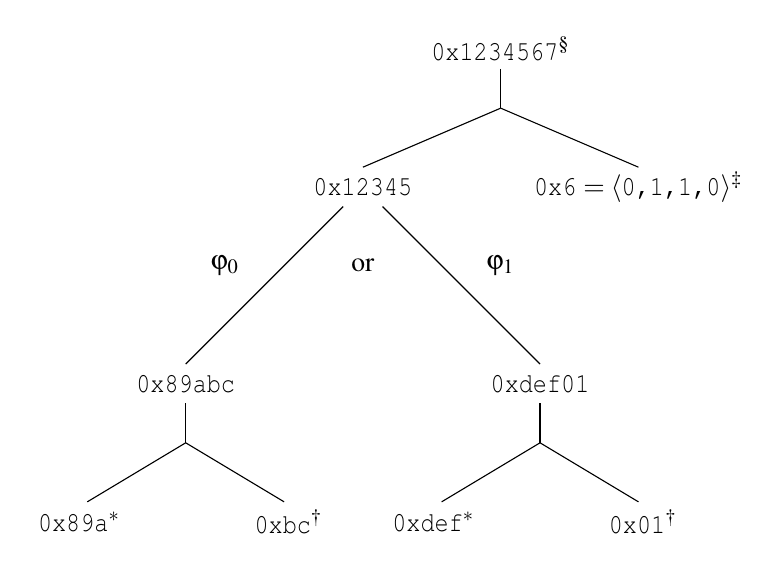
\begin{tikzpicture}

\draw (0,0) node[right] {{\tt 0x89a}$^{*}$};
\draw (0.75,0.25) -- (2.0,1.0);
\draw (2,1) -- (3.25,0.25);
\draw (2.75,0) node[right] {{\tt 0xbc}$^{\dag}$};

\draw (2,1) -- (2,1.5);
\draw (2,1.75) node {{\tt 0x89abc}};

\draw (4.5,0) node[right] {{\tt 0xdef}$^{*}$};
\draw (5.25,0.25) -- (6.5,1.0);
\draw (6.5,1) -- (7.75,0.25);
\draw (7.25,0) node[right] {{\tt 0x01}$^{\dag}$};

\draw (6.5,1) -- (6.5,1.5);
\draw (6.5,1.75) node {{\tt 0xdef01}};

\draw (2,2) -- (4.0,4);
\draw (6.5,2) -- (4.5,4);
\draw (2.5,3.25) node {$\varphi_0$};
\draw (4.25,3.25) node {or};
\draw (6,3.25) node {$\varphi_1$};
\draw (4.25,4.25) node {{\tt 0x12345}};

\draw (7.75,4.25) node {{\tt 0x6} $= \langle${\tt 0,1,1,0}$\rangle^\ddag$};

\draw (4.25,4.5) -- (6,5.25);
\draw (7.75,4.5) -- (6,5.25);
\draw (6,5.75) -- (6,5.25);
\draw (6,6) node {{\tt 0x1234567}$^\S$};
%\draw (0,0) to[out=0,in=90] (0.5,-0.5);
%\draw (0.5,-0.5) to[out=-90,in=0] (0.0,-1);
%\draw [-{Stealth[length=8, width=8]}] (0,-1) to[out=180,in=-90] (-0.5,-0.25);

%% \draw (6,0) node[left] {$\ge$ cursor, $\mathbb{Z}_2^{F-1}$, non-empty tail};
%% \draw (6,0) to[out=0,in=90] (6.5,-0.5);
%% \draw (6.5,-0.5) to[out=-90,in=0] (6.0,-1);
%% \draw [-{Stealth[length=8, width=8]}] (6,-1) to[out=180,in=-90] (5.5,-0.25);

%% \draw (2,2) node[left] {< cursor};
%% \draw (2,2) to[out=0,in=-90] (2.5,2.5);
%% \draw (2.5,2.5) to[out=90,in=0] (2.125,3);
%\draw [-{Stealth[length=8, width=8]}] (2.125,3) to[out=180,in=90] (1.75,2.25);

%% \draw [-{Stealth[length=8, width=8]}] (-1,0.25) to[bend left] (0.6,2);
%% \draw [-{Stealth[length=8, width=8]}] (-1,0.25) to[bend right] (1.1,1.75);
%% \draw [-{Stealth[length=8, width=8]}] (4,0.25) -- (1.75,1.75);

%% \draw (2.4,4.5) node[left] {$\ge$ cursor, $\mathbb{Z}_2^F$};
%% %\draw (1.6,4.5) node[left] {$\mathbb{Z}_2^9$};
%% \draw (2.4,4.5) to[out=0,in=-90] (2.9,5);
%% \draw (2.9,5) to[out=90,in=0] (2.525,5.5);
%% \draw [-{Stealth[length=8, width=8]}] (2.525,5.5) to[out=180,in=90] (2.15,4.75);

%% \draw [-{Stealth[length=8, width=8]}] (1.25,4.2) -- (1.25,2.25);
%% \draw [-{Stealth[length=8, width=8]}] (1.25,2.3) -- (1.25,4.25);

%\draw [-{Stealth[length=8, width=8]}] (-2,0.25) -- (0.5,4.25);
%\draw [-{Stealth[length=8, width=8]}] (5,0.25) -- (2,4.25);


%\draw (0,0)  (-0.5,-0.5);


%% \draw (0,0) rectangle (3,1);
%% \draw (-0.2,-0.8) node[right] {\Huge $\mathbb{Z}_2^{\lg (1^2 \pi^2 /6 \varepsilon)}$};

%% \draw (4,0) rectangle (7,1);
%% \draw (4,0) rectangle (7,-1);
%% \draw (3.8,-1.8) node[right] {\Huge $\mathbb{Z}_2^{\lg (2^2 \pi^2 /6 \varepsilon)}$};

%% \draw (8,1) rectangle (11,-3);
%% \draw (8,0) rectangle (11,-2);
%% \draw (8,-1) -- (11,-1);
%% \draw (7.8,-3.8) node[right] {\Huge $\mathbb{Z}_2^{\lg (3^2 \pi^2 /6 \varepsilon)}$};

%% \filldraw (11.5,0.5) circle (1pt);
%% \filldraw (12,0.5) circle (1pt);
%% \filldraw (12.5,0.5) circle (1pt);

%% \draw (13,1) rectangle (16,-1);
%% \draw (13,0) -- (16,0);
%% \filldraw (14.5,-1.5) circle (1pt);
%% \filldraw (14.5,-2) circle (1pt);
%% \filldraw (14.5,-2.5) circle (1pt);
%% \draw (13,-3) rectangle (16,-5);
%% \draw (13,-4) -- (16,-4);

%% \draw (10,-5.8) node[right] {\Huge$\mathbb{Z}_2^{\lg (\lceil\lg (n-1)\rceil^2 \pi^2 /(6 \varepsilon))}$};

%% \draw (16,-2) node[right]{\Huge$\left\}\begin{array}{c} \\ \\ \\ \\ \\ \\ \end{array}2^{\lceil \lg (n-1)\rceil-1}\right.$};


\end{tikzpicture}

\end{document}
